%%%%%%%%%%%%%%%%%%%%%%%%%%%%%%%%%%%%%%%%%%%%%%%%%%%%%%%%%%%%%%%%%%%%%%%%%%%%%%%%
%2345678901234567890123456789012345678901234567890123456789012345678901234567890
%        1         2         3         4         5         6         7         8

%\documentclass[letterpaper, 10 pt, conference]{orbieeeconfpre}  % Comment this line out if you need a4paper

\documentclass[a4paper, 10pt, journal]{wissarbIEEE}      % Use this line for a4 paper
%\conference{IEEE Conference for Awesome ORB Research}

\bibliographystyle{orbref-num}

\IEEEoverridecommandlockouts                              % This command is only needed if 
                                                          % you want to use the \thanks command

\overrideIEEEmargins                                      % Needed to meet printer requirements.

% See the \addtolength command later in the file to balance the column lengths
% on the last page of the document

\usepackage{hyperref}
\usepackage{graphicx}
\usepackage{tabularx}
\usepackage{booktabs}
\usepackage{lipsum}

\title{\LARGE \bf
Wissenschaftliches Arbeiten - \\Short paper \LaTeX\ document class*
}

\author{Guybrush U. Threepwood$^{1}$ and Alexander Schubert$^{2}$% <-this % stops a space
\thanks{*Based on the guidelines published on the \href{http://conf.papercept.net/conferences/support/tex.php}{PaperCept conference manuscript management website}}% <-this % stops a space
\thanks{$^{1}$Guybrush U. Threepwood is with the Institute for Pirate Sciences, Three-headed Monkey Group, University of  M\^el\'ee Island
        {\tt\small gthreepwood@har.har-har.mi}}%
\thanks{$^{2}$Alexander Schubert is with the Optimization in Robotics and Biomechanics Group, Institute of Computer Engineering, Heidelberg University, Berliner Str. 45, 69120 Heidelberg
        {\tt\small alexander.schubert@ziti.uni-heidelberg.de, \href{http://orb.iwr.uni-heidelberg.de}{orb.iwr.uni-heidelberg.de}}}%
}


\begin{document}



\maketitle

%%%%%%%%%%%%%%%%%%%%%%%%%%%%%%%%%%%%%%%%%%%%%%%%%%%%%%%%%%%%%%%%%%%%%%%%%%%%%%%%
\begin{abstract}

This demo file is intended to illustrate the short paper \LaTeX\ document class to be used for manuscripts created in the lecture `Wissenschaftliches Arbeiten' based on the style of IEEE publications.

\end{abstract}

%%%%%%%%%%%%%%%%%%%%%%%%%%%%%%%%%%%%%%%%%%%%%%%%%%%%%%%%%%%%%%%%%%%%%%%%%%%%%%%%
\section{The short paper document class}
{\bf Important!} Please note that the \verb!wissarbIEEE.cls! file is to be used within the context of the lecture {\it Wissenschaftliches Arbeiten} at the University Heidelberg only and must not be distributed externally!

%% Figure
\begin{figure}[h]
   \centering
   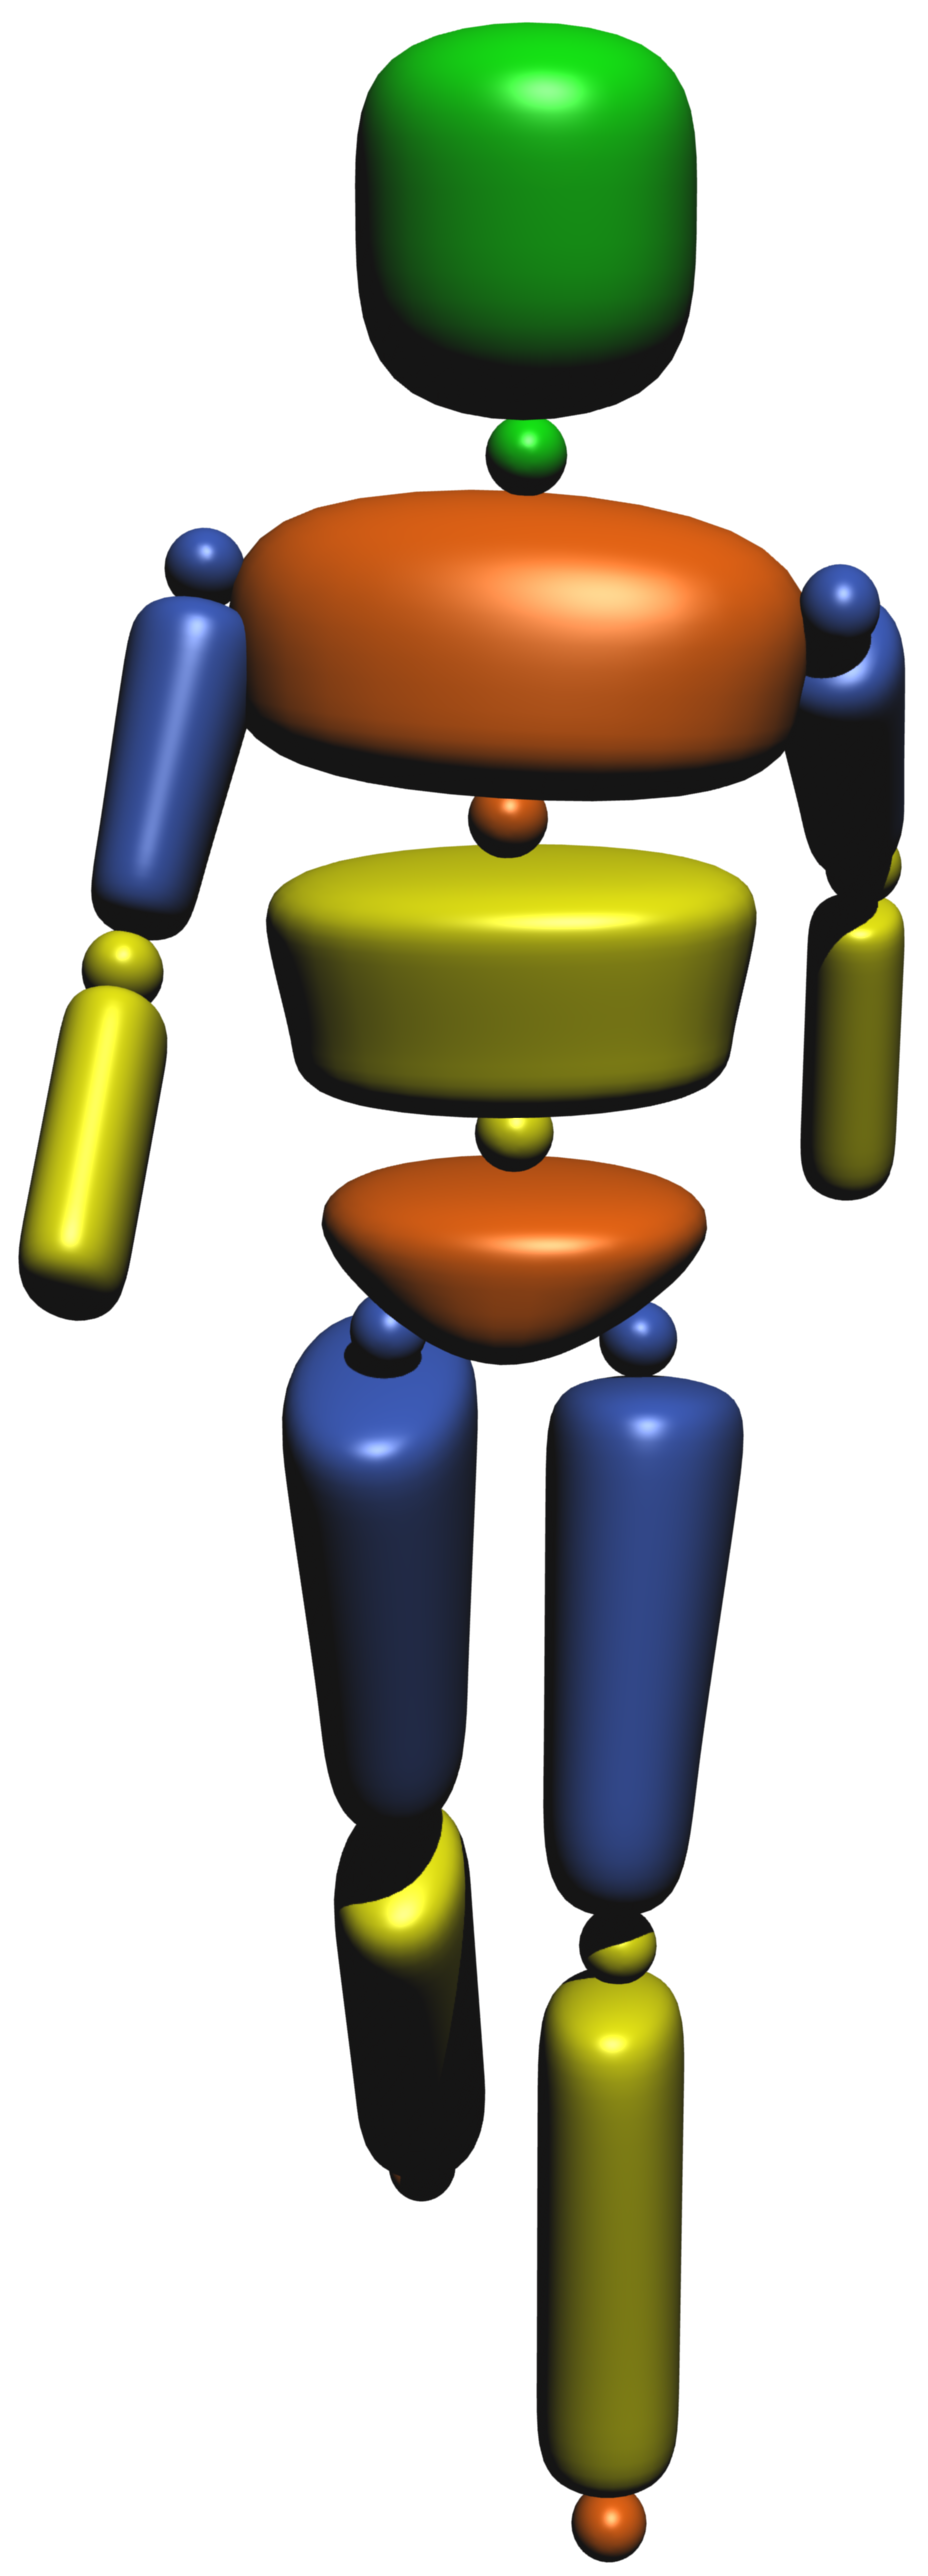
\includegraphics[width=0.1\textwidth]{fig/knubbi.png}
   \caption{Example picture.}
   \label{fig:knubbi}
\end{figure}

\subsection{Bibliography styles}
The \texttt{orbref-num.bst} bibliography style numbers the citations by their order of appearance. Here are two sample references: \cite{Newton1687,Mombaur2009}.

\subsection{Lorem Ipsum}
\lipsum[1]

%% Table
\begin{table}[h]
\caption{Example table.}
   \begin{tabularx}{0.48\textwidth}{llr}
   		 \toprule 
   		 Symbol & \multicolumn{1}{X}{Description} & Value [m] \\
		 \midrule
		  $A_x$ & Horizontal coordinate of A$^{*}$ & 0.0745 \\
		  $A_z$ & Vertical coordinate of A$^{*}$ & 0.2650 \\  \noalign{\smallskip}
		  
		  $C_x$ & Horizontal coordinate of C$^{\#}$ & 0.0700 \\
		  $C_z$ & Vertical coordinate of C$^{\#}$ & 0.1000 \\
		  $D_x$ & Horizontal coordinate of D$^{\dag}$ & 0.0602 \\
		  $D_z$ & Vertical coordinate of D$^{\dag}$ & 0.0860 \\
		 \bottomrule
   \end{tabularx}  \label{tab:initmodel}
\end{table}

\lipsum[2]

\bibliography{mybibfile}

\end{document}
